\documentclass[preprint,12pt]{article}

\usepackage{algorithmic}
\usepackage{algorithm}
\usepackage{enumerate}
\usepackage{enumitem}
\usepackage{graphics}
\usepackage{graphicx}
\usepackage{geometry}
\usepackage{amsmath}
\usepackage{wrapfig}
\usepackage{subfig}
\usepackage{framed}
\usepackage{color}
\usepackage{soul}
\usepackage{bm}

\usepackage{natbib}
\usepackage{multirow}
\usepackage[T1]{fontenc}
\usepackage[latin9]{inputenc}
%\usepackage{units}
\usepackage{esint}
\geometry{legalpaper,  margin=1in}

\newcommand{\CM}[2][green]{ {\sethlcolor{#1} \hl{#2}} }
\newcommand{\KB}[2][cyan]{ {\sethlcolor{#1} \hl{#2}} }
%THIS IS TO PUT ALL FLOATS AT THE END OF THE DOC SO THEY CAN BE SPLIT INTO A SEPARATE FILE
%%\usepackage{endfloat}
%\makeatother

%\usepackage{babel}

\begin{document}
\title{An Empirical Bayesian Framework for Assessing Partisan Bias in Redistricting Plans}

\author{Kevin Baas and Colin McAuliffe}

\maketitle


\section{Partisan Bias in the Wisconsin State Assembly, post 2010 census\label{sec:Wis}}

\begin{figure}[htb!]
    \begin{center}
        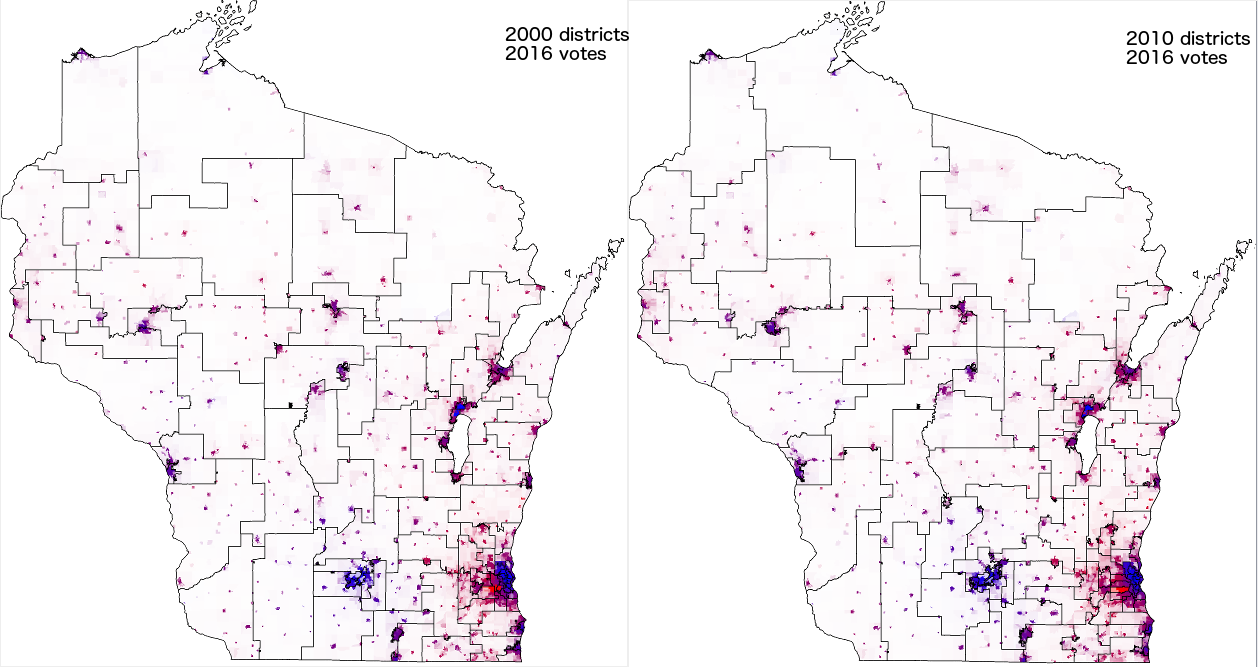
\includegraphics[scale=0.35]{../../Figures/WI_compared/precincts_pop_combined.png}
        \caption{2016 Assembly election results by precinct, projected onto Assembly districts before and after Act 43. Left: 2000 cycle districts, Right: 2010 cycle districts}\label{fig:MapsWI}
    \end{center}
\end{figure}

The Wisconsin state assembly districts are the subject of \emph{Whitford v. Gill}, where a federal court has ruled that the redistricting plan is an unconstitutional gerrymander.
The plaintiffs in \emph{Whitford} relied on the efficiency gap to demonstrate bias, while here we apply the expected specific asymmetry.

Some have alleged that the bias in the Wisconsin map is merely the product of changes in voter sentiment and/or political geography.
The argument that there is a natural packing of Democratic voters in urban areas is stated in the Amicus Brief filed by the Republican National Committee and the National Republican Congressional Committee.
The tendency of Democratic voters to cluster in urban areas is well known, but no proof was offered to suggest that the electoral advantage given to Republicans in the Act 43 map was merely the result of this effect and not of deliberate gerrymandering, nor was this ever claimed.
Furthermore, supporters of defendants never argued that partisan gerrymandering due to political geography should not be or cannot be neutralized.
The RNC and NRCC brief, however, argues that doing so would result in "bizarrely shaped districts", though they provide no evidence to support this claim, and this claim is directly contradicted by maps supplied to the court in plaintiffs' initial filing.

The RNC and NRCC brief cited the studies of Chen and coworkers, among others, in support of the notion that gerrymandering can occur unintentionally due to population clustering \cite{Chen_2015_10.1089/elj.2015.0317,Chen_2016_10.1016/j.electstud.2016.06.014}.
In one of these papers \emph{cited in the Amicus Brief}, Chen and coworkers say that an additional partisan bias of roughly 4\% of the total available seats in Wisconsin districts is \emph{not} explainable by political geography.

A more recent study of the Act 43 map by Chen \cite{Chen_2017_} found that out of 200 computer-generated maps -- which made no effort to minimize partisan bias --  \emph{all of them} were significantly \emph{less} "bizarrely shaped" than the Act 43 districts \emph{and} had significantly less partisan bias.
73\% of them had an efficiency gap within 3\% of zero, and 10\% of them had an efficiency gap favoring \emph{Democrats}.
The study concluded:

\emph{"Act 43 not only created an extremely biased Assembly plan with an efficiency gap far outside of any gap observed in 200 simulations, the enacted plan achieved this partisan outcome at the expense of traditional districting principles, splitting apart far more counties and municipalities than were necessary."}

The fact that the Act 43 map does not attempt to preserve existing political boundaries directly undercuts the argument that the bias in the map arises from natural political geography.
And the fact that it has a significantly higher efficiency gap than any of these computer-generated maps -- 10\% of which favor Democrats -- supports the opposite conclusion: \emph{Act 43} districts are more "bizarrely shaped" than district plans with a \emph{lower} efficiency gap.

In what follows, we employ a different analysis methodology and find that the Act 43 map leads to an increase in seats won by Republican candidates by increasing the partisan asymmetry in their favor relative to the previous map.
This is further evidence that the bias in the Act 43 map reflects the deliberate intentions of the redistricters, and simply can not be explained by political geography alone.

To compare how much of the observed partisan asymmetry in 2010-cycle Wisconsin State Assembly districts was the result of changes in district designs versus changes in voter sentiment, we projected actual election results onto both the current Assembly districts, and Assembly districts from the previous redistricting cycle, as shown in figure \ref{fig:MapsWI}.
This allows us to analyze the effects of changes in voter sentiments and redistricting separately.

For this analysis we used official districting plans for the 2000 and 2010 census cycles, and actual vote counts from the 2006, 2008, 2010, 2012, 2014, and 2016 assembly elections, at precinct-level resolution, imputing uncontested elections with partisan swing matched presidential election results when available, and partisan swing matched federal congress election results when not.
By "partisan swing matched" we mean that the Republican vote counts in all districts are multiplied by a constant factor so that the total vote count matches that for the assembly elections, for the subset of districts in which both elections were contested, and the same is done for the Democratic vote counts.
Then election data for 2006, 2008, and 2010 were cross-aggregated at census block resolution to the 2010-cycle districts, and election data for 2012, 2014, and 2016 were cross-aggregated at census block resolution to the 2000-cycle districts. 
Since the same exact elections are used in both the 2000 districts analysis and 2010 districts analysis, \emph{all} differences in the results are the consequence of the redistricting scheme used, and conversely, changes in voter sentiment have exactly \emph{zero} contribution to the difference.

If the 2000 census cycle districts show a partisan asymmetry much lower than the 2010 cycle, then we would know that natural "political geography" -- the tendency of Democratic voters to be clustered in cities -- can be immediately ruled out as a significant factor in the partisan asymmetry inherent in 2010 cycle Wisconsin Assembly districts, since any contributions from political geography would be present in \emph{both} districting schemes.
However if they are not substantially different, this would not demonstrate that political geography was a significant contribution, because they both could be artificially gerrymandered on top of any unintentional gerrymandering due to political geography.
In this case, further analysis would be required to separate the effects of unintentional bias caused by political geography and deliberate bias caused by gerrymandering.

\subsection{Observed partisan asymmetries in past elections}

\begin{figure}[htb!]
    \begin{center}
        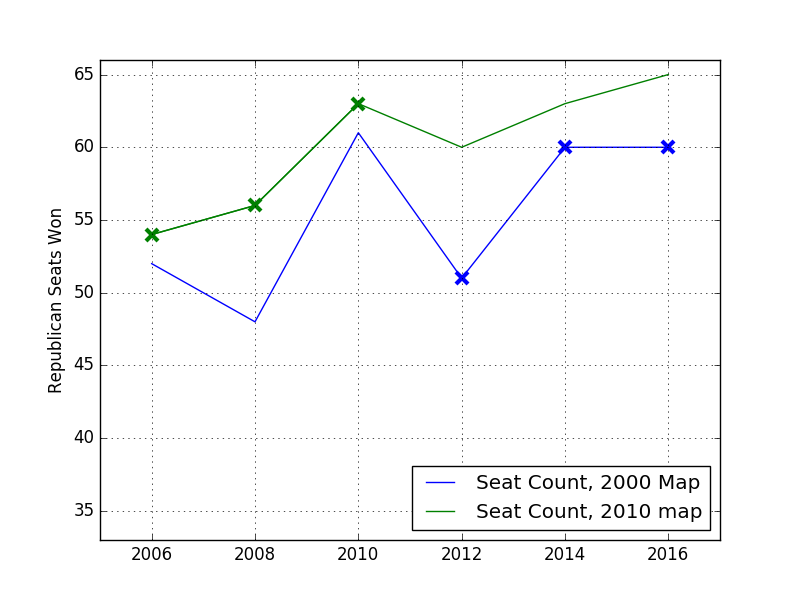
\includegraphics[scale=0.85]{../../Figures/WI2010/WI_2000_2010_seats.png}
        \caption{Republican Seat Counts in Assembly elections, using 2000 cycle districts vs 2010 cycle districts. The X's indicate that a result has been cross aggregated, meaning results were computed on a different district map than the one that actually existed at the time of the election.}\label{fig:Seats20002010}
    \end{center}
\end{figure}

\begin{figure}[htb!]
    \begin{center}
        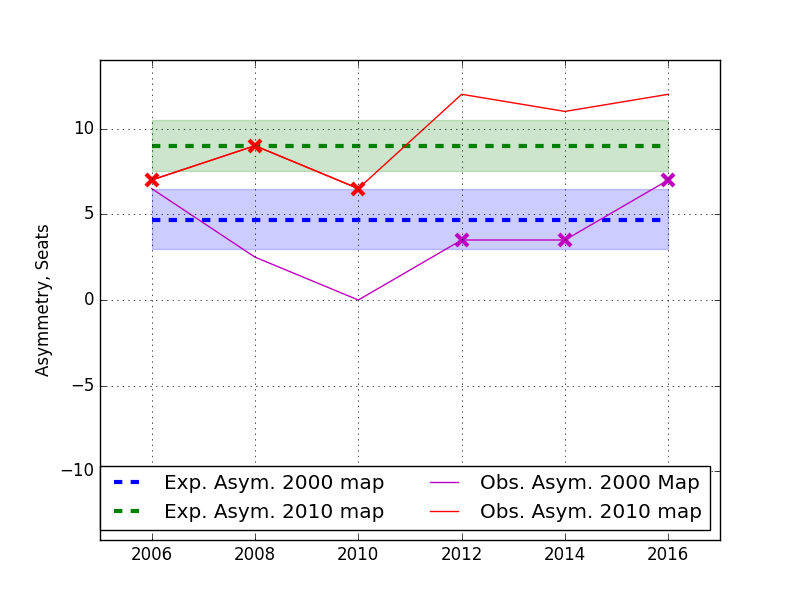
\includegraphics[scale=0.85]{../../Figures/WI2010/WI_2000_2010.png}
        \caption{Historical asymmetry in Assembly elections, using 2000 cycle districts vs 2010 cycle districts. The X's indicate that a result has been cross aggregated, meaning results were computed on a different district map than the one that actually existed at the time of the election.  The dashed lines represent the statistical expectations, and the shaded areas represent the 50\% confidence intervals.}\label{fig:Asym20002010}
    \end{center}
\end{figure}

After imputing uncontested elections and projecting onto the two different districting schemes, we counted up the wins and computed the specific asymmetry for each election on each map.
The seat counts are shown in figure \ref{fig:Seats20002010}, and the specific asymmetry is shown in figure \ref{fig:Asym20002010}.  They are also tabulated in table \ref{tab:seats}.
The horizontal lines and shaded regions represent the statistical expectation and 50\% confidence intervals, respectively.

The charts show a clear and stable separation between both seat counts and partisan asymmetry between 2000 districts and 2010 districts.
They both go up and down largely in parallel, responding about the same to changes in voter sentiment.
This tells us that in the 2012, 2014, and 2016 elections, the new districts led to an increase in Republican representation over what the old districts would have produced.
Furthermore, were the new districts used in the 2000 redistricting cycle, that would have produced about the same increase in Republican representation for the 2006, 2008, and 2010 elections.

\begin{table}[htb!]
\centering
\caption{Summary of the differences in seat counts and asymmetries for elections on the two legislative maps \label{tab:seats}}
\begin{tabular}{|l|l|l|l|}
\hline
Election Year & Rep. Seats, 2000 Map & Rep. Seats, 2010 Map & Net Change in Seats\\
\hline
\hline
2006 & 52 & 54 & R + 2\\
\hline
2008 & 48 & 56 & R + 8\\
\hline
2010 & 61 & 63 & R + 2\\
\hline
2012 & 51 & 60 & R + 9\\
\hline
2014 & 60 & 63 & R + 3\\
\hline
2016 & 60 & 65 & R + 5\\
\hline
\hline
Election Year & Asymmetry, 2000 Map & Asymmetry, 2010 Map & Net Change in Asymmetry\\
\hline
\hline
2006 & 6.5 & 7.0 & R + 0.5\\
\hline
2008 & 2.5 & 9.0 & R + 6.5\\
\hline
2010 & 0.0 & 6.5 & R + 6.5\\
\hline
2012 & 3.5 & 12.0 & R + 8.5\\
\hline
2014 & 3.5 & 11.0 & R + 7.5\\
\hline
2016 & 7.0 & 12.0 & R + 5.0\\
\hline
\end{tabular}
\end{table}


In figure \ref{fig:Asym20002010diff}, the difference in seats won by Republicans is plotted along with the difference in the expected asymmetries between the two maps.
The increase in seats gained by Republicans in the 2010 map is entirely explained by the increase in asymmetry in the 2010 map.
Therefore the 2010 map leads to greater Republican representation by \emph{structurally disadvantaging Democratic voters}.


\begin{figure}[htb!]
    \begin{center}
        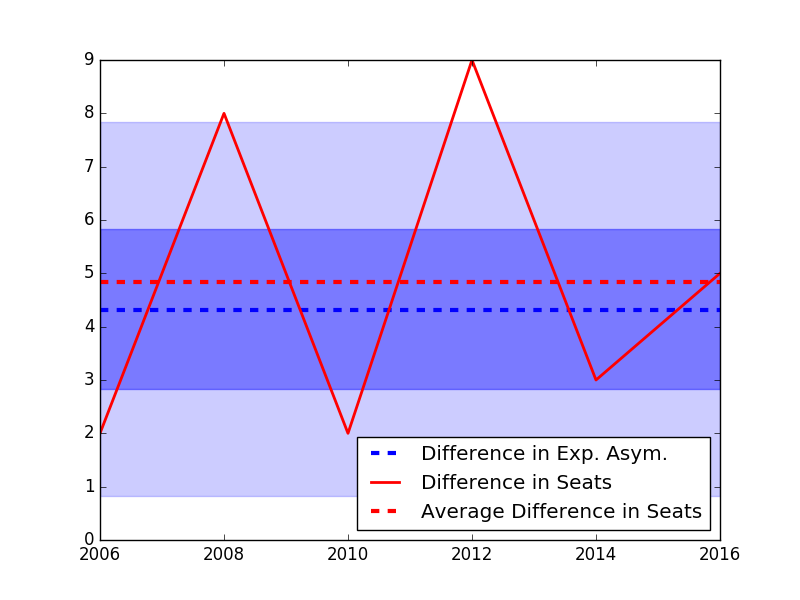
\includegraphics[scale=0.85]{../../Figures/WI2010/WI_2000_2010diff.png}
        \caption{Difference in seats won by Republicans in the two maps. The dashed blue line shows the difference in expected asymmetry between the two maps, the blue and light blue shaded regions represent 50\% and 90\% confidence intervals}\label{fig:Asym20002010diff}
    \end{center}
\end{figure}

\begin{figure}[htb!]
    \begin{center}
        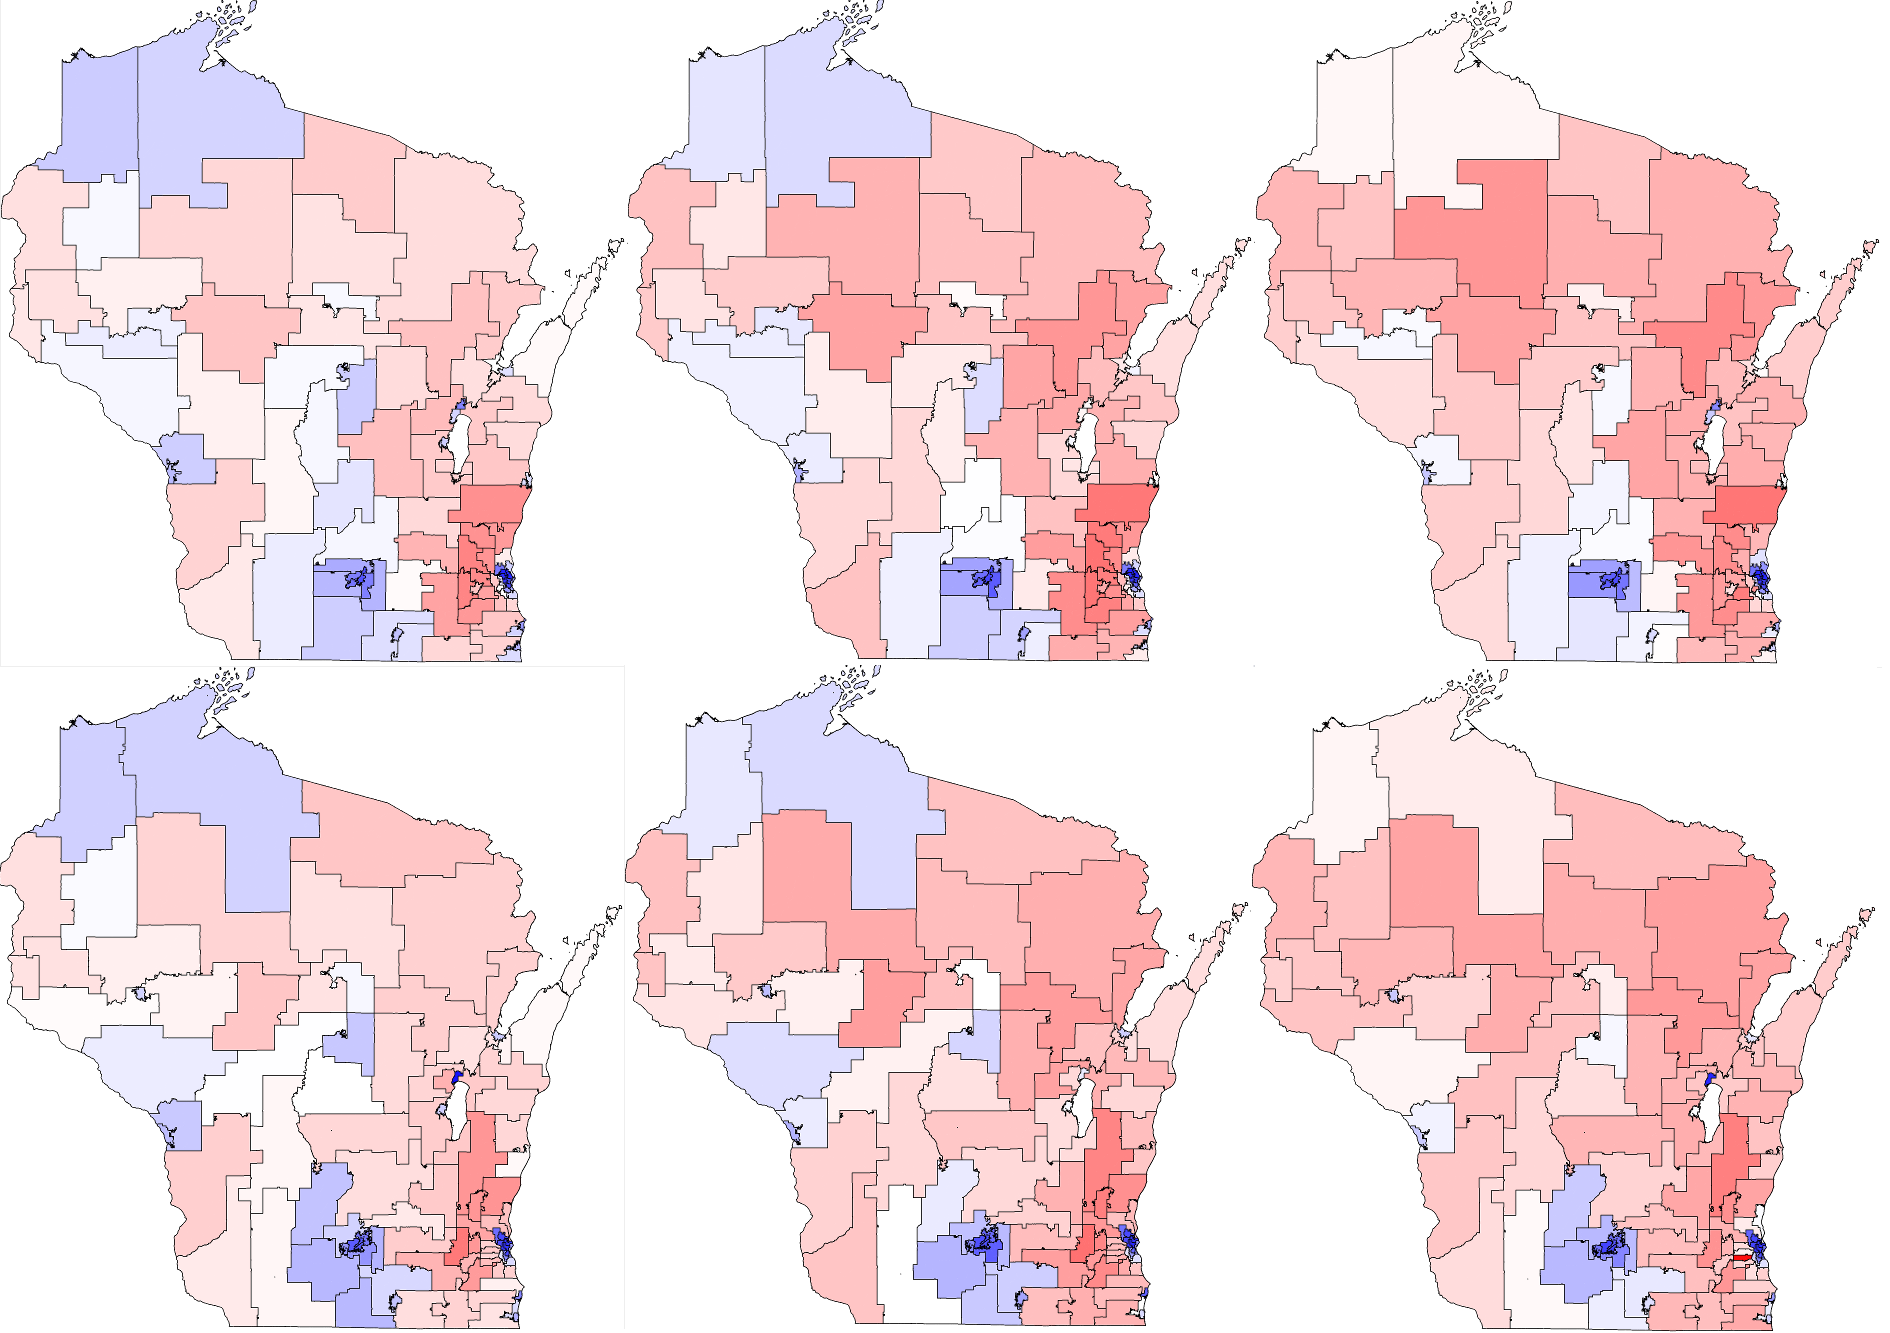
\includegraphics[scale=0.25]{../../Figures/WI_compared/3x2.png}
        \caption{Partisan vote packing in Wisconsin Assembly elections. Top: 2000 cycle districts, Bottom: 2010 cycle districts, Left to right: 2012, 2014, and 2016 elections.}\label{fig:DistrictMaps}
    \end{center}
\end{figure}


We can better visualize how the 2010 districts give Republicans more seats than the 2000 districts by coloring in the districts according to the victory margin, and comparing.
Figure \ref{fig:DistrictMaps} shows such a comparison for 2012, 2014, and 2016 elections (left to right).
The two Democratic districts above Lake Winnebago were combined into one, taking a seat away from Democrats.
Democratic voters in Eau Claire once participated in two competitive districts, which would have given Democrats 2 seats with 2000 district lines, but the 2010 district lines wrapped them up in a single safe district, capping the number of elections those voters can swing at 1.
In 2000 districts, Madison is surrounded by several competitive Democratic-leaning districts.
But the 2010 lines packed Democratic voters surrounding Madison into a few safe Democratic districts, flipping the districts those voters came from, which would have been competitive, to Republican.
In Milwaukee, the lines were redrawn to more tightly outline Democratic voters, thus creating a few more districts that Republicans can win in.
Indeed, figure \ref{fig:DistrictMapDelta} shows that by comparing the districting schemes using 2016 votes, it is easy to identify where Republicans picked up 4 seats due to partisan vote packing.

Simultaneously, deeper red districts throughout the state were redrawn to give away some of their Republican voters to nearby competitive districts, reducing the likelihood that a Democratic representative would be elected in the once-competitive districts while still maintaining a safe edge in the originally deeper red district.  
You can see this by noticing the much "flatter" red color in the bottom maps versus the top maps.
It will also be made clear in the next subsection when we examine the statistical properties of the maps more rigorously.

In sum, the changes in the district lines from 2000 districts to 2010 districts consist of decreasing the number of Democratic districts through vote packing, and increasing the number of Republican districts through vote cracking.
Instances of the reverse (packing Republican voters and cracking Democratic districts) are simply not present.
\begin{figure}[htb!]
    \begin{center}
        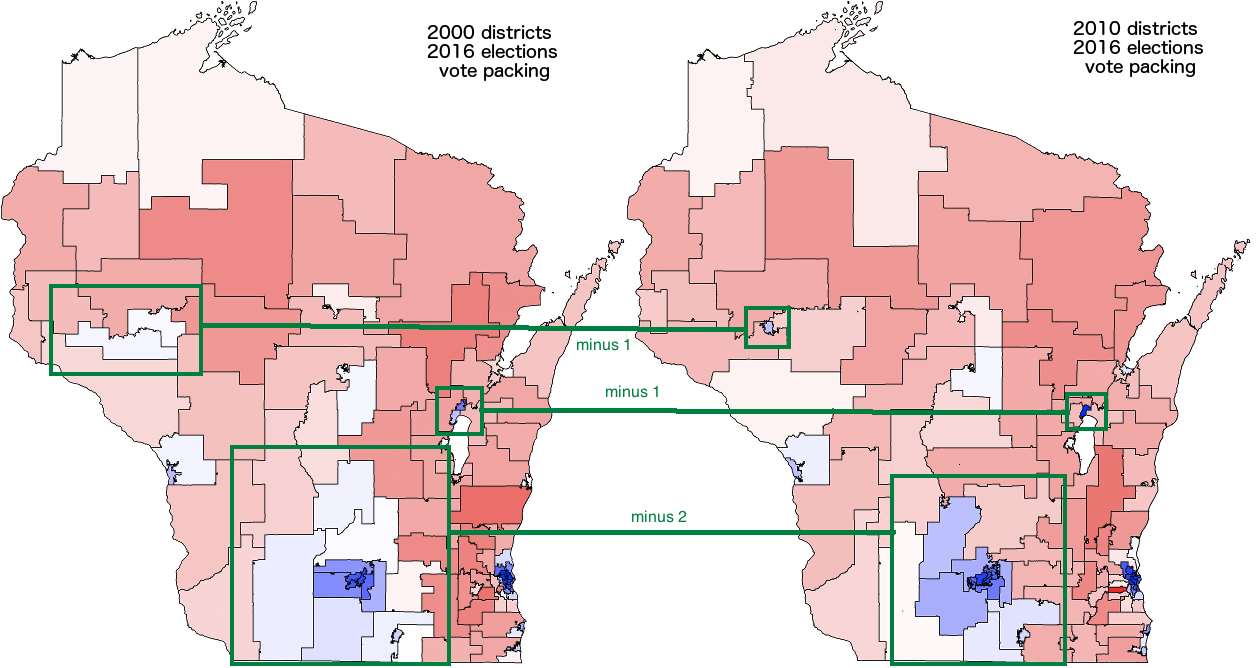
\includegraphics[scale=0.40]{../../Figures/WI_compared/districts_compared_deltas.png}
        \caption{Partisan vote packing in Wisconsin Assembly elections, using 2016 election data.  Outlined in green are areas where Republicans packed Democratic votes.}\label{fig:DistrictMapDelta}
    \end{center}
\end{figure}



\subsection{Expected  partisan asymmetries in future elections}

\begin{figure}[htb!]
    \begin{center}
        \includegraphics[scale=0.25]{../../Figures/WI_compared/Betas_cropped.png}
        \caption{Beta distributions for Wisconsin 2010-cycle Assembly districts, Top: 2000 cycle districts, Bottom: 2010 cycle districts}\label{fig:BetasWI}
    \end{center}
\end{figure}
 
Figure \ref{fig:BetasWI} shows the beta distributions estimated for each district and the popular vote under the 2000 and 2010 redistricting plans. 
Before evaluating this model with Monte Carlo sampling, we can find some clear signs of pro-Republican gerrymandering just from inspection of these distributions. 
Many Republican-leaning districts are tightly clustered at levels of partisanship that allow Republican candidates to win safely without wasting too many votes, while many Democrat-leaning districts are heavily packed and not competitive.
In the 2010, distributions Republicans-leaning districts are more concentrated around a single point slightly but safely short of competitive, while Democratic-leaning districts that were competitive in the 2000 distributions have been shifted away from the center.
Consequently, in the 2010 distributions, compared to the 2000 distributions, Republicans are expected to gain more seats by smaller margins, while Democrats are expected to gain fewer seats by larger margins.


\subsubsection{Specific partisan asymmetry likelihoods}
 
The results of Monte Carlo integration are shown in figure \ref{fig:LikelihoodsAsymmetry}, as a fraction of total available seats.  
The graph shows the seat \emph{gap} -- the difference between the seats-votes curve and it's reflection at the statewide popular vote -- so dividing by 2 gives the asymmetry.
These results were also used to compute the expectations and confidence intervals shown in figures \ref{fig:Asym20002010} and \ref{fig:Asym20002010diff}.
 
\begin{figure}[htb!]
    \begin{center}
        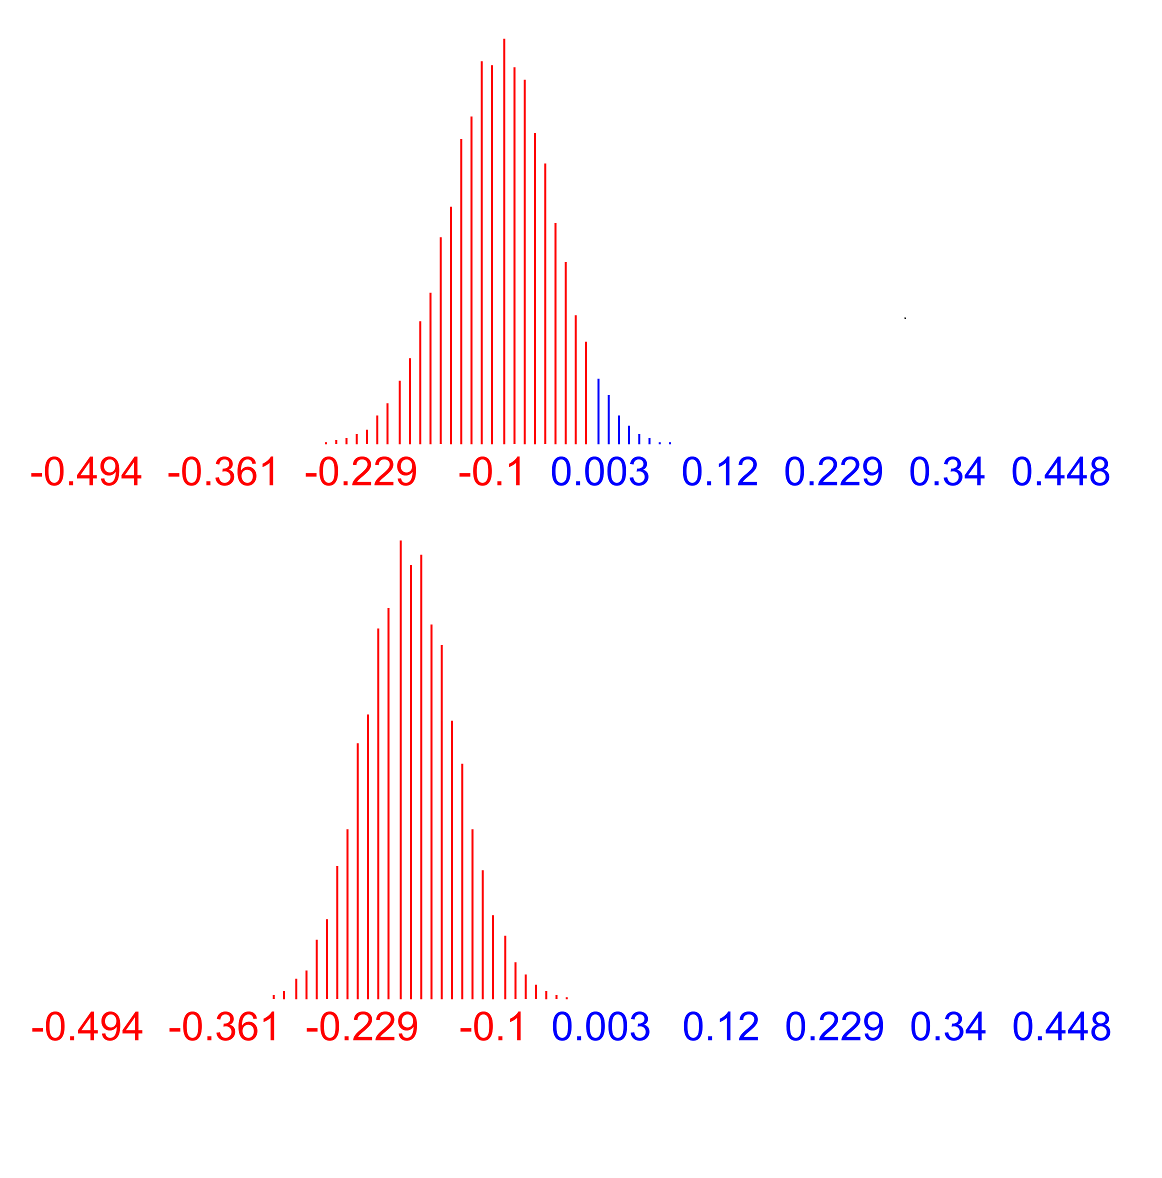
\includegraphics[scale=0.25]{../../Figures/WI_compared/asymmetry_cropped.png}
        \caption{Specific asymmetry likelihoods, Top: 2000 cycle districts, Bottom: 2010 cycle districts}\label{fig:LikelihoodsAsymmetry}
    \end{center}
\end{figure}
 
For the 2000 districts, the partisan asymmetry favors Republicans, giving them an average seat boost of 5\% of the available seats beyond what a symmetric seats-votes curve would produce.  
However, there is still a decent likelihood that voter sentiments would change enough that Democrats would get a small boost from seats-votes curve asymmetry.

For the 2010 districts, the partisan asymmetry favors Republicans by twice the amount of the 2000 districts, giving them an average seat boost of 10\% of the available seats beyond what a symmetric seats-votes curve would produce.  
The most likely result in the Wisconsin state assembly might be that Republicans get 6/10ths of the legislative seats, whereas if the popular vote count were reversed, Democrats would get only 4/10th of the legislative seats.  
Remedying this would give Democrats 10\% more seats.  
This means that roughly 10\% of the entire Democratic-voting population of the state of Wisconsin were effectively disenfranchised, in violation of the one person, one vote principle.  
Conversely, 10\% of the Republican-voting population effectively got an extra vote, which is approximately equivalent to 306,000 cases of illegal voting.
This is a very large gerrymander relative to what was found in our examination of U.S. congress.

Unlike the 2000 districts, out of 100,000 samples drawn, \emph{none} of them resulted in specific partisan asymmetry favoring Democrats.  
Since an assembly district election occurs every 2 years, this shows that, without significant changes in geo-spatial demographics, the asymmetric pro-Republican partisan advantage inherent in this redistricting will persist for the next 200,000 years.

\subsubsection{District partisanship histogram}
  
\begin{figure}[htb!]
    \begin{center}
        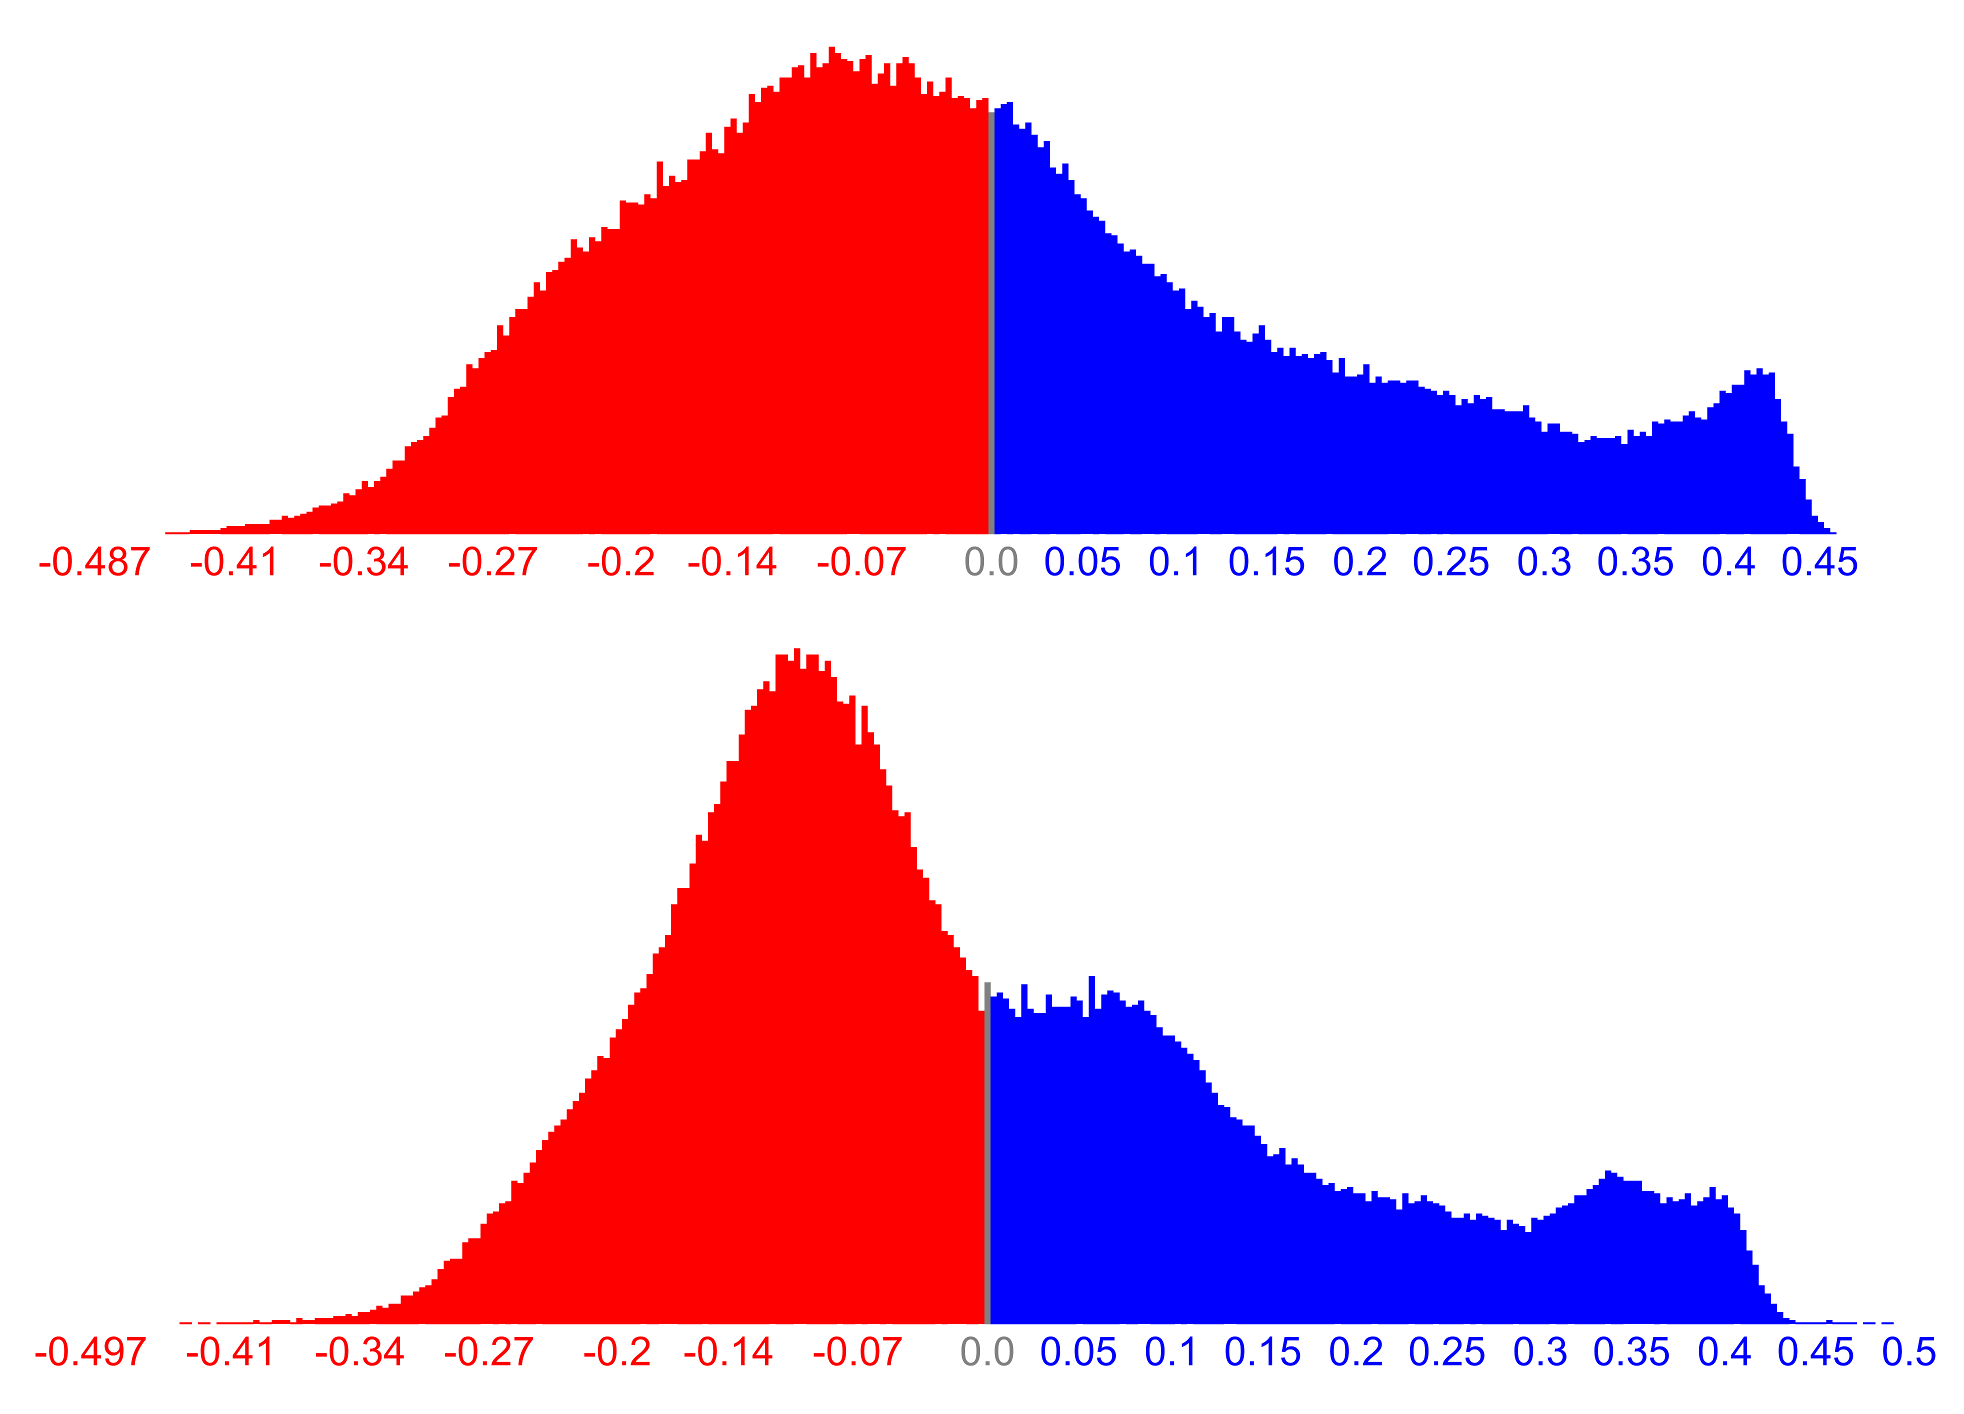
\includegraphics[scale=0.25]{../../Figures/WI_compared/district_partisanship_cropped.png}
        \caption{District partisanship likelihoods, Top: 2000 cycle districts, Bottom: 2010 cycle districts}\label{fig:LikelihoodsDistrictPartisanship}
    \end{center}
\end{figure}

Another way we can visualize the partisan asymmetry in the Wisconsin state assembly map is by looking at the histogram of district partisanship.
The same Monte Carlo integration technique we used to compute the expected specific asymmetry can be used to construct the likelihood function for district partisanship over all districts and all possible election outcomes.
In other words, if one were to pick a random district in a random election, this curve shows how likely the vote in that district is to be 25\% Republican vote, a 50-50 split, etc.
 
The curve for the 2000 districts show a smooth peak near 50/50, with a slight skew towards Republicans and a long tail on the Democratic side with a brief peak at the end.  
This shows that Democratic districts were packed, while Republican districts were cracked.

On the other hand the curve for the 2010 districts show a much sharper distinction.
It has a high red peak close to the center but still safely to the side, that already drops off sharply by the time it hits 50/50, and then on the blue side, drops slowly all the way until it gets to a larger bump at the extremely packed end of the scale.
This clearly reveals that Republican candidates in Republican leaning districts have a high likelihood of winning safely but without wasting too many votes, while Democratic candidates in Democratic leaning districts have a high likelihood winning by margins that waste a lot of votes.
You can also see this effect visually on the maps in figure \ref{fig:DistrictMaps}: the red colors are much "flatter" in 2010 districts (bottom) than 2000 districts (top).

\subsubsection{Statewide seat count likelihoods}

\begin{figure}[htb!]
    \begin{center}
        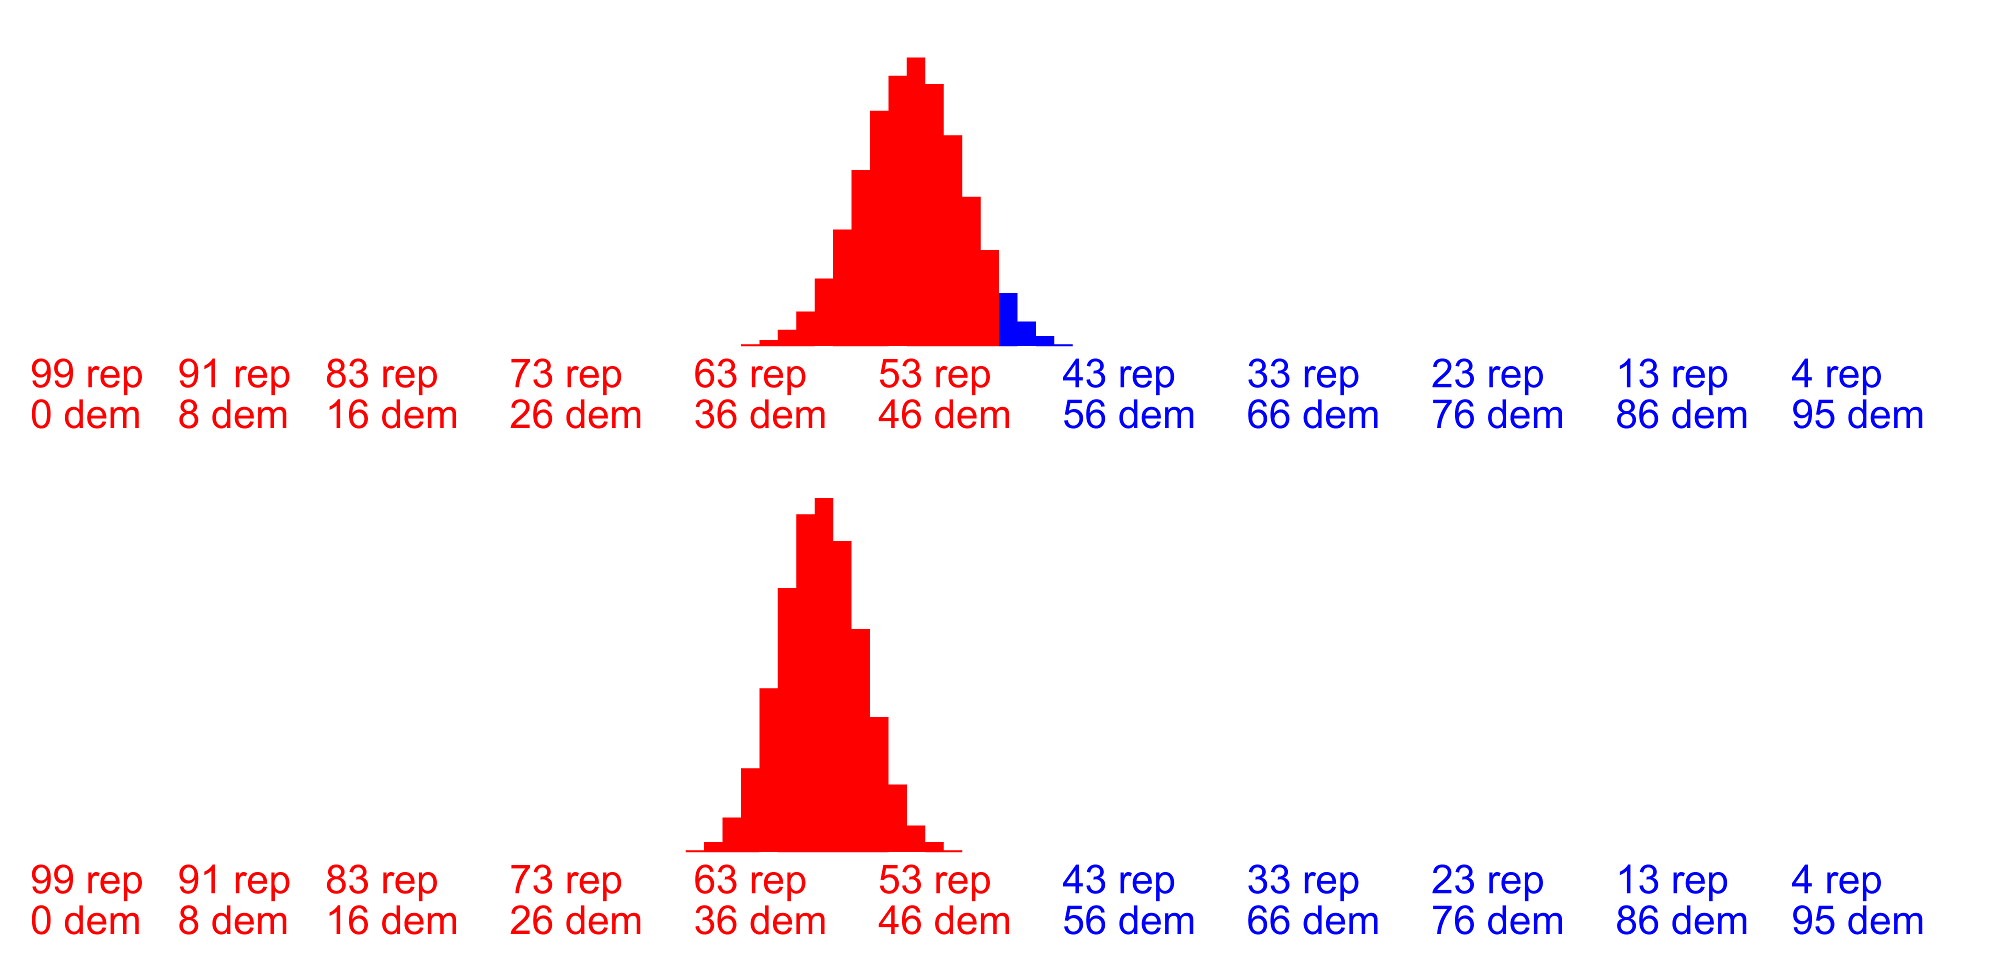
\includegraphics[scale=0.25]{../../Figures/WI_compared/seats_cropped.png}
        \caption{Seat count likelihoods, Top: 2000 cycle districts, Bottom: 2010 cycle districts.}\label{fig:LikelihoodsSeatCounts}
    \end{center}
\end{figure}
 
A third way to use the Monte Carlo results to understand asymmetry is to estimate the likelihood of every possible election outcome, district-by-district.
We then accumulate these outcomes on a chart, with the seat count on one axis, and the likelihood on the other.  The results are shown in figure \ref{fig:LikelihoodsSeatCounts}.

In 2000 districts, the expected outcome is for Republicans to win a 54-45 majority of seats, though Democrats still have a decent chance of winning the majority of seats. 
In 2010 districts, Republican's expected lead grows by an additional 10 seats to 59-40. 
Despite being favored by roughly half the voters, Democrats have no chance at all to win a majority of seats even in the most eccentric swings of voter sentiment.
Out of 100,000 samples, Democrats rarely even get 45 of the seats, which was their average under the 2000 districting scheme.

\subsection{Discussion}

Measured by partisan asymmetry, both expected and observed, there was substantial gerrymandering in favor of Republicans in the 2000 cycle maps.
This asymmetry leads to about 4 extra Republican seats beyond what would be allocated if the seats-votes curve was symmetric.
The current method does not distinguish what part of this gerrymandering was deliberate and what part unintentional, though regardless of the proportion, it is trivial to generate a map without this asymmetry by using one of many well-known optimization algorithms. 
Indeed, recent simulations by Jowei Chen \cite{Chen_2017_} show that there is a good chance of generating a partisanly neutral map \emph{unintentionally}.

If we disregard data that was not available when the 2010 cycle districts were drawn, and use only data from the 2006, 2008, and 2010 elections, we see that with the new redistricting lines, Republicans are expected to gain an additional 4 assembly seats (an 8 seat swing), beyond what the previous (2000 cycle) redistricting lines would have given them.
Furthermore, this is in addition to the partisan asymmetry already present in the 2000 cycle maps, bringing the expected total seat difference gained over Democrats through partisan asymmetry to 18.

The fact that the 2010 cycle maps have double the partisan asymmetry as the 2000 maps demonstrates that regardless of what part of the gerrymandering in the 2000 cycle maps was deliberate, \emph{at least} half of the gerrymandering in the 2010 cycle maps was deliberate.
In any case, a map optimized by a computer algorithm to maximize partisan symmetry could remove almost all of the deliberate gerrymandering, and at least some of the unintentional gerrymandering.

From these comparisons, it is clear that the specific partisan asymmetry present in the 2010 cycle districts is \emph{not} present in the 2000 cycle districts, even when using vote count data from the exact same elections.  Therefore:
\begin{itemize}

\item The difference between the two schemes is a stable 10\% gain in the Republican seat margin over Democrats.
Since the same exact voter sentiments were used in both analyses, this difference in partisan asymmetry simply cannot be a consequence of changes in voter sentiment.  
Since the only thing that we changed was the districting scheme, all observed differences in partisan asymmetry are purely the result of changing the districting scheme and reflect the choices made by the redistricters and do not reflect changes in political geography.
\item Claims that the election results it produced are similiar to those under the previous districts are categorically false.
\item In order to claim that natural political geography was a significant factor in the 2010 cycle district, we would expect to see the exact same asymmetries in the 2000 districts.
To the contrary, partisan asymmetry in 2010 districts is double that of 2000 districts, even after compensating for observed and potential changes in voter sentiment.
\item Claims that the observed partisan bias in 2010 districts is simply a consequence of political geography and/or changes in voter sentiment are contradicted by this analysis.
\item Simply reverting back to the 2000 census cycle districts would remedy most of the present injustice, as measured in seats affected or ballots affected.
\end{itemize}

This comparison cannot estimate how much of the gerrymandering present in the 2000 districts was deliberate.
However it does demonstrate that the 2010 districts, under the same elections, give Republicans more seats than the 2000 districts, and that this difference will persist even in the most extreme swings of voter sentiment.

\section{Conclusions}
An empirical Bayesian framework for analyzing partisan bias in redistricting plans was presented, along with a new metric for gerrymandering called the specific asymmetry.
The metric is an effective measure of redistricting bias, and is consistent with existing opinions by the Supreme Court since it does not rely on proportionality or hypothetical results.
The empirical Bayesian model allows one to asses the likelihood of a given redistricting plan causing partisan asymmetry and harm to voters in future elections, which permits an analyst to distinguish between observations of bias which occurred by chance on a fair map and maps for which bias is a persistent feature.

This technique was applied to U.S. congress for elections from 1972 to 2016, and substantial levels of asymmetry were found.
The total amount of asymmetry favoring both parties combined in each cycle has held fairly constant, although the 2010 cycle is remarkable since many states appear to be moving toward more symmetric districting plans, while simultaneously several states (especially those known to have been targeted by the REDMAP project) have unprecedented levels of asymmetry.
We also analyzed the Wisconsin state assembly map under Act 43 and the map for the 2000 cycle, where we found that the Act 43 map roughly doubled the level of asymmetry from the previous map, and that this increase in asymmetry can not be explained by political geography as supporters of defendants in \emph{Whitford v. Gill} have alleged.


\clearpage
\section*{Acknowledgment}
\section*{}
\bibliographystyle{unsrt}
\bibliography{gerrymandering}
\clearpage



\end{document}
